\documentclass{article}

\usepackage{fullpage}
\usepackage{color}
\usepackage{amsmath}
\usepackage{url}
\usepackage{verbatim}
\usepackage{graphicx}
\usepackage{parskip}
\usepackage{amssymb}
\usepackage{nicefrac}
\usepackage{listings}


% Colors
\definecolor{blu}{rgb}{0,0,1}
\def\blu#1{{\color{blu}#1}}
\definecolor{gre}{rgb}{0,.5,0}
\def\gre#1{{\color{gre}#1}}
\definecolor{red}{rgb}{1,0,0}
\def\red#1{{\color{red}#1}}
\def\norm#1{\|#1\|}

% Math
\def\R{\mathbb{R}}
\def\argmax{\mathop{\rm arg\,max}}
\def\argmin{\mathop{\rm arg\,min}}
\newcommand{\mat}[1]{\begin{bmatrix}#1\end{bmatrix}}
\newcommand{\alignStar}[1]{\begin{align*}#1\end{align*}}
\def\half{\frac 1 2}

% LaTeX
\newcommand{\fig}[2]{\includegraphics[width=#1\textwidth]{#2}}
\newcommand{\centerfig}[2]{\begin{center}\includegraphics[width=#1\textwidth]{#2}\end{center}}
\newcommand{\matCode}[1]{\lstinputlisting[language=Matlab]{a2f/#1.m}}
\def\items#1{\begin{itemize}#1\end{itemize}}
\def\enum#1{\begin{enumerate}#1\end{enumerate}}

\def\rubric#1{\gre{Rubric: \{#1\}}}{}

\begin{document}

\title{CPSC 340 Assignment 2}
\author{Henry Deng \\ Student Number: 41584103}
\date{}
\maketitle
\vspace{-4em}

\section{Naive Bayes}

\subsection{Naive Bayes by Hand}
\rubric{reasoning:3}

(a)
\items{
\item$ p(y = 1) = 0.6$
\item $p(y = 0) = 0.4$
}

(b)
\items{
\item $p(x_1 = 1 | y = 1) = \frac{1}{2}$
\item $p(x_2 = 0 | y = 1) = \frac{1}{3}$
\item $p(x_1 = 1 | y = 0) = 1$
\item $p(x_2 = 0 | y = 0) = \frac{3}{4}$
}

(c) 
\items{
\item $p(\hat{y} = 0|\hat{x}) \propto p(\hat{x_1} = 1|\hat{y} = 0) * p(\hat{x_2} = 0|\hat{y} = 0) * p(\hat{y} = 0)$ = $1 * \frac{3}{4} * 0.4 = 0.3$
\\
\item $p(\hat{y} = 1|\hat{x}) \propto p(\hat{x_1} = 1|\hat{y} = 1) * p(\hat{x_2} = 0|\hat{y} = 1) * p(\hat{y} = 1)$ = $\frac{1}{2} * \frac{1}{3} * 0.6 = 0.1$
}
\vspace{3mm}
\hspace{5mm} \blu{Naive bayes predicts $\hat{y} = 0$ since $p(\hat{y} = 0|\hat{x})$ is bigger than $p(\hat{y} = 1|\hat{x})$}


\subsection{Bag of Words}

\enum{
\item league 
\item car, engine, evidence, problem, system
\item 2
}

\subsection{Naive Bayes Implementation}

\begin{verbatim}
https://github.ugrad.cs.ubc.ca/CPSC340-2017W-T2/c1z8_a2/blob/master/code/naive_bayes.py
\end{verbatim}
Test error after the fix is $0.188$ 
\\ The accuracy of the validation error is close to sklearn's value of $0.187$, but a little off from the random forest value of $0.197$. 

\subsection{Laplace smoothing}

1. Refer to: 

\url{https://github.ugrad.cs.ubc.ca/CPSC340-2017W-T2/c1z8_a2/blob/master/code/naive_bayes.py}


\enum{
\item[2] I had to modify my fit function 
\item[3] The scikit version uses the default value of $\alpha = 1$ for Laplace smoothing. When I passed in $\beta = 1$, I got the same result as the scikit version. 
}

\subsection{Runtime of Naive Bayes for Discrete Data}

The cost of classifying t test examples is $O(tdk)$

\section{Random Forests}

\subsection{Implementation}

\enum{
\item The random tree does not have a training error of 0 because we only randomly sample a small number of features, which may not cover all possible number of features, so we will never overfit the data regardless of the depth of the tree. 
\item Refer to: \url{https://github.ugrad.cs.ubc.ca/CPSC340-2017W-T2/c1z8_a2/blob/master/code/random_forest.py}
\item Fig 1. Decision Tree vs. Random Tree vs. Random Forest. \\ \hspace{45mm} 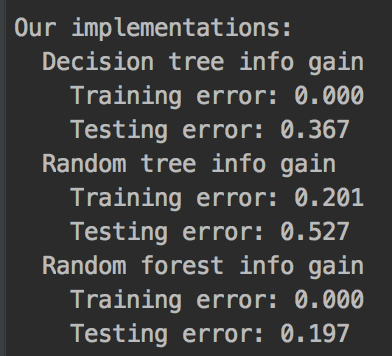
\includegraphics[scale=0.5]{../figs/forest_example.png} \\ 
Yes. These results are expected because decision trees overfit and therefore, have a training error of 0 and a high test error. A random tree cannot cover all features so the training and test errors are high. When we increase the number of random trees into a forest, we cover more features and avoid overfitting; therefore, train error and test error are reduced dramatically.  
\item Our implementation was much slower than scikits RandomForestClassifier, but accuracy was similar with our testing error clocked at $0.197$ and scikit's testing error at $0.186$. 
}


\subsection{Very-Short Answer Questions}

\enum{
\item One disadvantage is the increase in calls to the random forest classifier, which could lead to a bad running time.
\item 
\enum{
\item Decrease the maximum depth of the trees in your forest.
\item Decrease the amount of data you consider for each tree. 
\item Decrease the number of features you consider for each tree.
}
\item Add transformed data during training, ie. warping the audio to create multiple versions of the audio
}


\section{Clustering}

\subsection{Selecting among $k$-means Initializations}

\enum{
 \item Refer to: \url{https://github.ugrad.cs.ubc.ca/CPSC340-2017W-T2/c1z8_a2/blob/master/code/kmeans.py}
 \item The value of the k-means error decreases and then stabilizes 
 \item Plot is provided here: \\
 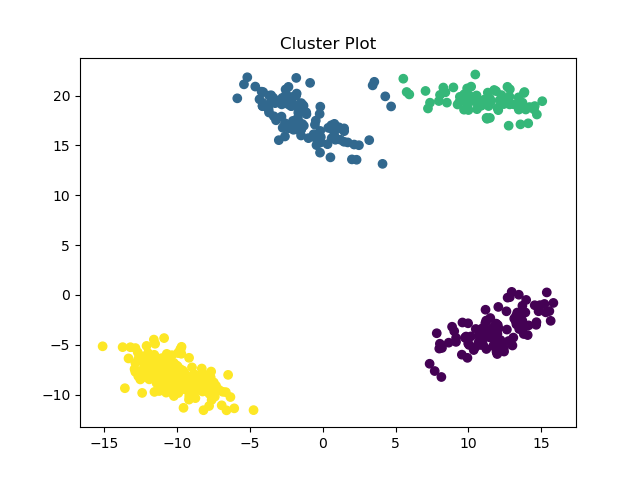
\includegraphics[scale=0.6]{../figs/kmeans_lowest_error.png} \\ 
 Fig. 2: Plot of the clustering obtained by running k-means 50 times and taking the lowest error
 \item n-clusters = number of clusters, init = used to increase values, n-init = number of initializations, max.iterations = how many times you run kmeans 
 }


 \subsection{Selecting $k$ in $k$-means}

\enum{
 \item The error function will keep decreasing as k increases. Therefore, we will always select the largest value of k, which is not a suitable method to select k.
 \item If we increase the value of k, we will get more clusters in our test data. As we increase in clusters, the mean of each cluster is going to be closer to the true value of each point. This can lead to overfitting of our data, so the error function is not suitable for selecting k even with test data. 
 \item Attached Plot: \\
  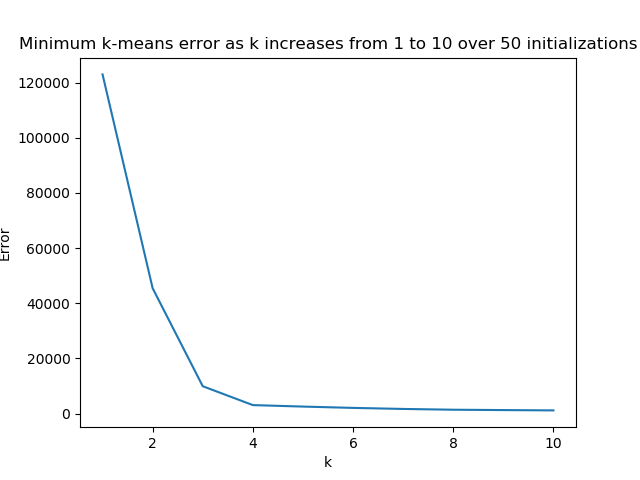
\includegraphics[scale=0.6]{../figs/kmeans_errors.png} \\ 
   Fig. 3: Plot of the minimum error found across 50 random initializations 
 \item Looking at the plot, the elbow method would select k = [2, 3, 4]. I would personally choose k = 3 due to the decreased error.
 }

 \subsection{$k$-medians}

\enum{
 \item The result is not satisfactory because the plot is an example of bad clustering since the outliers are not detected; thus, resulting in high error \\
 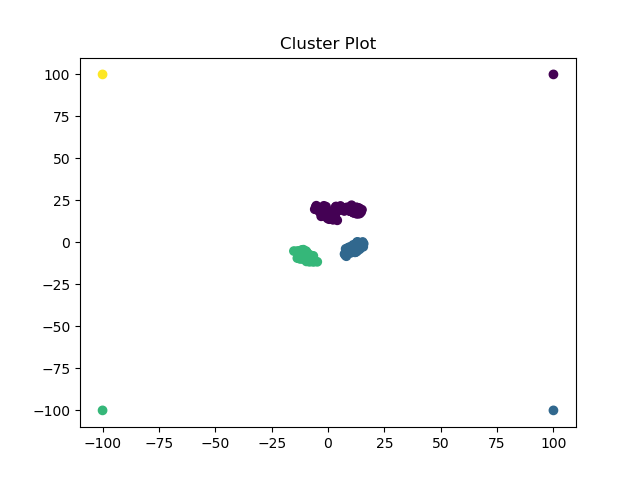
\includegraphics[scale=0.6]{../figs/cluster_kmeans_error.png} 
 \item The elbow method would select k = [2, 4, 8] since they have the steepest slopes. \\
  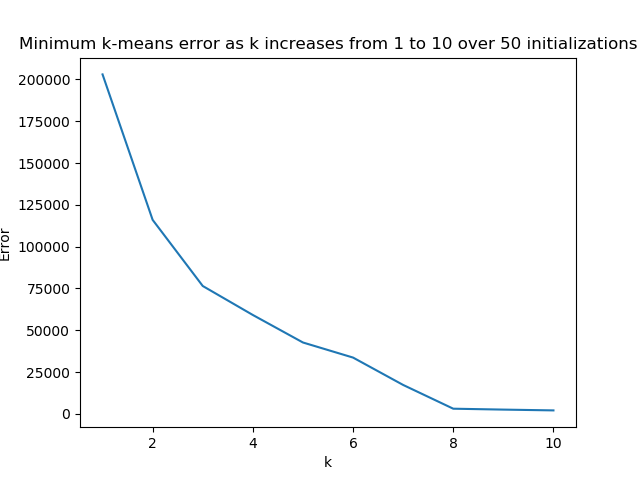
\includegraphics[scale=0.6]{../figs/cluster_errors.png} 
 \item Refer to:  \url{https://github.ugrad.cs.ubc.ca/CPSC340-2017W-T2/c1z8_a2/blob/master/code/kmedians.py}
 Plot: \\
   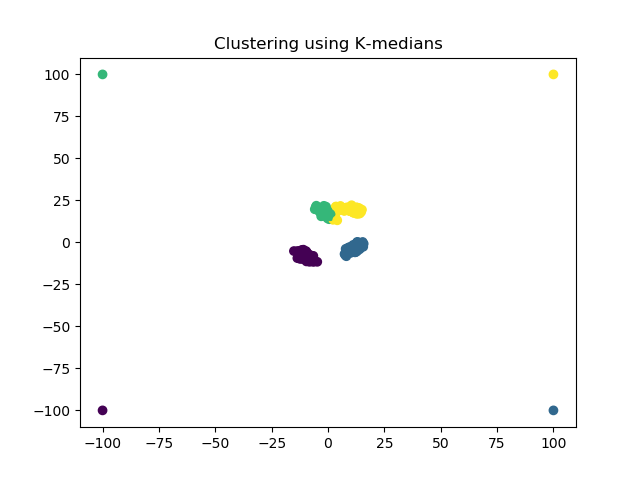
\includegraphics[scale=0.6]{../figs/kmedians_lowest_error.png} 
\item This time, the elbow method would select k = [2, 3, 4] since they have the steepest slopes. Yes, I am satisfied with this result since it is similar to the k-means result back in subsection 3.2. The variance in selecting k has decreased dramatically, which is a good thing. \\
   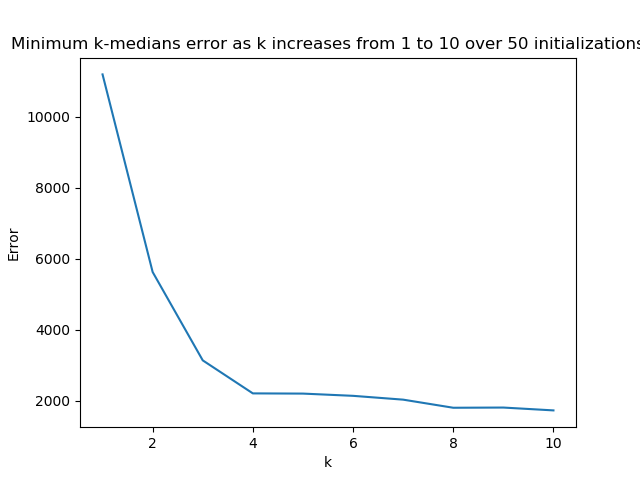
\includegraphics[scale=0.6]{../figs/k_medians_cluster_errors.png} 
}


\subsection{Density-Based Clustering}

{\enum{
\item eps = 2, minPts = 2
\item eps = 4, minPts = 2
\item eps = 15, minPts = 2
\item eps = 20, minPts = 2 
}

\subsection{Very-Short Answer Questions}

\enum{
\item No, depends on the initial clusters. 
\item When k = n. This value is not useful because we could have imperfect clustering but perfect test data. 
\item Hierarchical clustering would make it hard for k-means to find the true clusters 
\item This would affect the core assignment because there's different weights associated with kilograms vs. milligrams  
\item The key advantage of supervised outlier detection is that we know what the outliers could be, so we can detect them. The disadvantage is that we might not be able to detect new outliers.
}


\section{Vector Quantization}

\enum{
\item Refer to: \url{https://github.ugrad.cs.ubc.ca/CPSC340-2017W-T2/c1z8_a2/blob/master/code/quantize_image.py}
\item Quantization bit = 1, 2, 4, and 6 respectively shown below in order: \\
 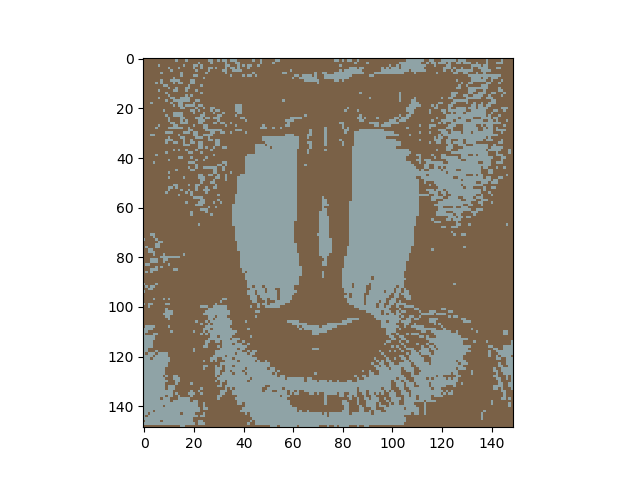
\includegraphics[scale=0.6]{../figs/b_1_image.png} \\
 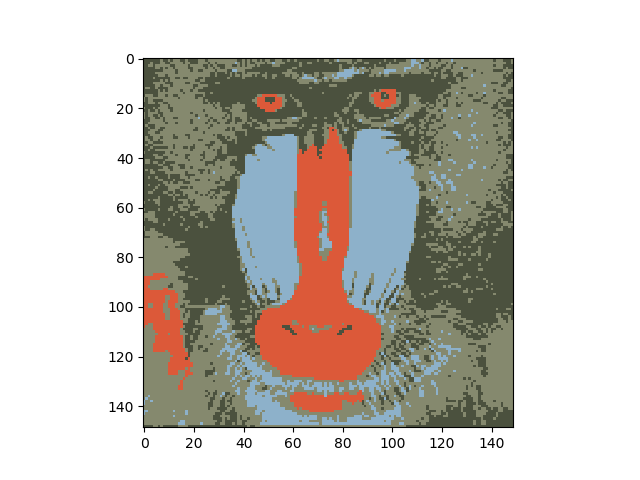
\includegraphics[scale=0.6]{../figs/b_2_image.png} \\
 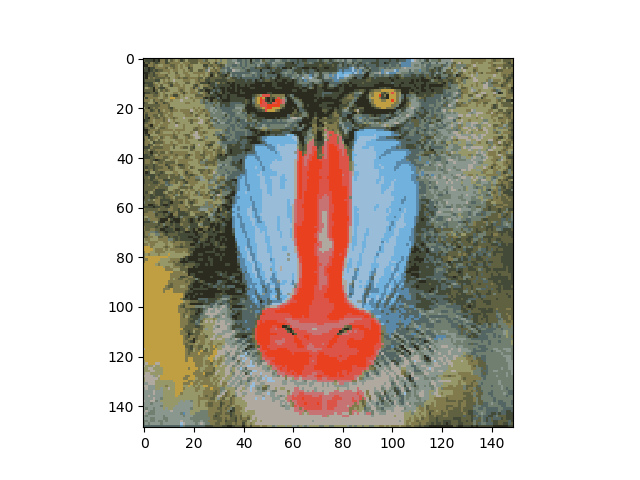
\includegraphics[scale=0.6]{../figs/b_4_image.png} \\
 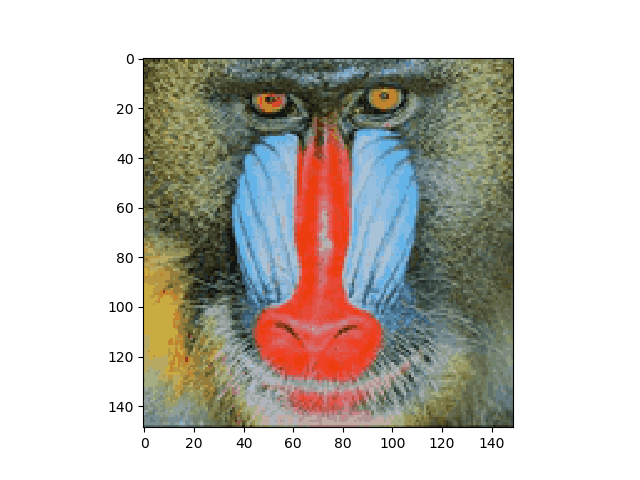
\includegraphics[scale=0.6]{../figs/b_6_image.png} \\
\item At each phase, we learn $2^b$ colours -- where b is the number of bits. When b = 6, we have learned most of the colours which is why the image looks very similar to the original image. 
}

\end{document}
